\chapter{Motivation}

Als Fake News werden Falschmeldungen bezeichnet, die mit manipulativer Absicht viral verbreitet werden. In dem 
"Whitepaper"\cite{facebook}, was Facebook am 27.04.2017 veröffentlichte, werden vier verschiedene Motive und  
Methoden von Falschnachrichten beschrieben. Zum einen mit der Absicht anhand von Fake News politische Stimmungen 
zu steuern, zum anderen mithilfe von Fehlinformationen bestimmt Gefühle zu erzeugen oder Aufmerksamkeit zu erzielen. 
Ein weitere Methode kann das manipulieren von politischen Diskussionen mithilfe von koordinierten Aktivitäten sein und 
zu letzt die bloße Desinformation.

Die Motive und Methoden werden immer komplexer und aufgrund der hohen Lukrativität\cite{Cynk} wird es immer schwieriger 
ohne große Eigenrecherche zu erkennen, ob die Nachricht der Wahrheit entspricht oder eine Falschmeldung ist.
Da eine Verbreitung in sozialen Netzwerken deutlich einfacher ist und diese Platformen zunehmend als einzige
Informationsquelle genutzt werden, wächst die Gefahr die von Fake News ausgeht.
Auch die Verbreitung von Nachrichten ist in sozialen Netzwerken deutlich leichter und Falschmeldungen sind schwer 
zu revidieren. 
Daher besteht ein großes Interesse darin, schnell zu wissen, ob Nachrichten der Wahrheit entsprechen oder nicht, um 
eine Verbreitung früh zu unterbinden. 

Eine Überprüfung des Inhalts würde zu viel Zeit in Anspruch nehmen. Eine schnellere Möglichkeit wäre eine Analyse 
des Textes mithilfe von Natural Language Processing und Neuronal Networks.
Dabei werden sowohl Kontext als auch Schreibstil des Textes analysiert und dann anhand dieser Information eine 
Likelihood bestimmt zu der ein Text "Fake" oder "Real" ist.
Diese Methode kann eine Überprüfung des Inhalts nicht ersetzen, 
jedoch könnte es bei einer ausreichenden Genauigkeit zu einem vorläufigen Sperren der Nachricht führen, was die 
unaufhaltsame Verbreitung dieser Falschmeldung verhindern würde.

Eine schon vorhandene Möglichkeit Fake News zu detektieren ist der "B.S. Detector" von Daniel Sieradski\cite{BS}.
Diese Browser Erweiterung überprüft alle verlinkten Webseiten auf verdächtige Quellen, indem es die Domains 
mit einer manuell gepflegten Liste von unzuverlässigen Quellen vergleicht. Dieses Tool hat das Problem, dass 
die Liste manuell geführt werden muss und es durch Vermeiden der fragwürdigen Domains möglich ist, den Filter zu 
umgehen. 

\chapter{Struktur und Verarbeitung des Datensatzes}

Der Datensatz besteht zu $44\%$ aus Nachrichten die vom B.S. Detektor detektiert wurden und zu $56\%$ aus gesammelten 
Nachrichten von vertrauenswürdigen Nachrichtendiensten, wie die Washington Post oder die New York Times. Die Nachrichten 
sind hauptsächlich auf Englisch und die Falschnachrichten sind vom 25.Oktober.2016 bis 25.November.2016 gesammelt worden. Für den Zeitraum 
der Real News ist Oktober bis November 2016 angegeben. 
Der Fake News Datensatz ist auf Kaggle.com zu finden\cite{fake_data} und die Real News werden in einem Kernel hinzugefügt\cite{real_data}.
Nach Aussortieren der nicht englischsprachigen Texte mithilfe der \textsc{langdetect}-Bibliothek\cite{langdetect}, welche die
Language Detection Bibliothek von Google\cite{google_langdetect} nutzt, hat der gesamte Datensatz eine Größe von 
$\num{27903}$.

Aufgrund des gegebenen Datensatzes kann die Fragestellung dieser Arbeit nur eingeschränkt formuliert werden.
Mithilfe dieses Datensatzes kann keine allgemeine Fake News Erkennung trainiert werden, da hier nicht der Inhalt 
ausschlaggeben für die Klassifizierung der Trainingsdaten ist, sondern der B.S. Detektor und somit die Quellen des 
Artikels. 
Zudem gibt es in dem Real News Datensatz nur $10$ verschiedene Herausgeber.
Daher hat der Datensatz eine große Verzerrung und es kann nur darauf trainiert werden, ob Texte vom B.S. Detektor 
als fragwürdig klassifiziert werden würden oder ob sie von einem der $10$ als glaubwürdig erachteten Herausgebern stammt.

Zunächst wird der Datensatz mithilfe der \textsc{nltk}-Bibliothek\cite{nltk} durch Lemmatisierung verarbeitet, um 
alle Wörter auf ihre Stammform zurückzuführen. 
Anschließend werden die Worthäufigkeiten in jedem Text mithilfe der \textsc{scikit-learn}-Bibliothek\cite{scikit-learn} 
gezählt. 
Somit ergibt sich das Bag-of-words Modell als Repräsentation des Textes.
Auf eine Aussortieren der Stoppwörter wird verzichtet, da diese zwar nicht relevant für den Inhalt der Nachricht sind,
jedoch Teil des Schreibstils sind und somit relevant für eine Trennung sein können.

\begin{comment}
    \begin{figure}[t!]
    \centering
    \begin{subfigure}[t]{0.45\textwidth}
        \centering
        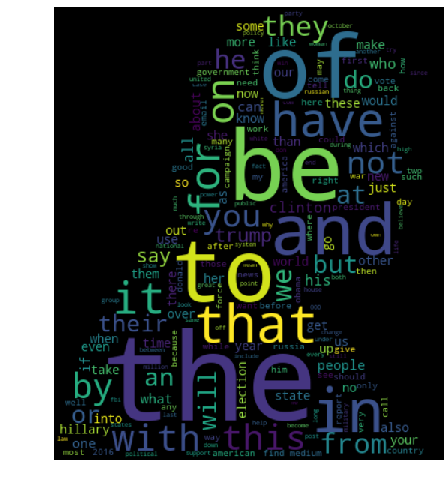
\includegraphics[width=\textwidth]{pictures/fake_wordcloud.pdf}
        \caption{Fake News}
    \end{subfigure}
    \begin{subfigure}[t]{0.54\textwidth}
        \centering
        \raisebox{1.5cm}[0pt]{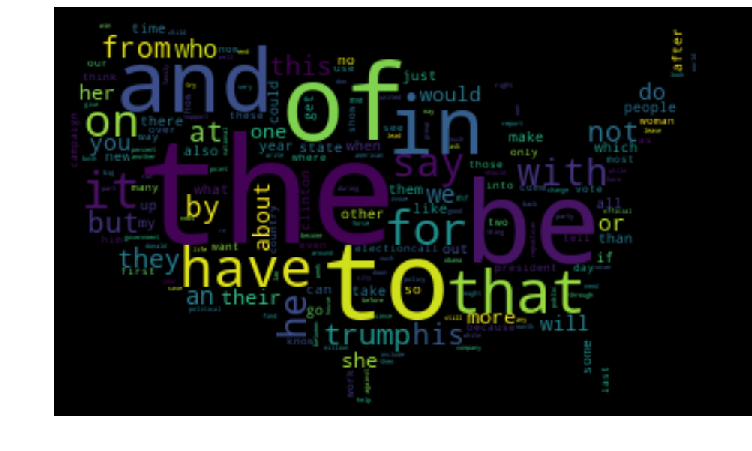
\includegraphics[width=\textwidth]{pictures/real_wordcloud.pdf}}
        \caption{Real News}
    \end{subfigure}
    \caption{Mit \textsc{wordcloud} \cite{wordcloud} erstellte Darstellung der Worthäufigkeiten für Real und Fake News.}
    \label{fig:wordcloud}
    \end{figure}
\end{comment}



\chapter{Lösungsansatz}

\begin{figure}
    \centering
    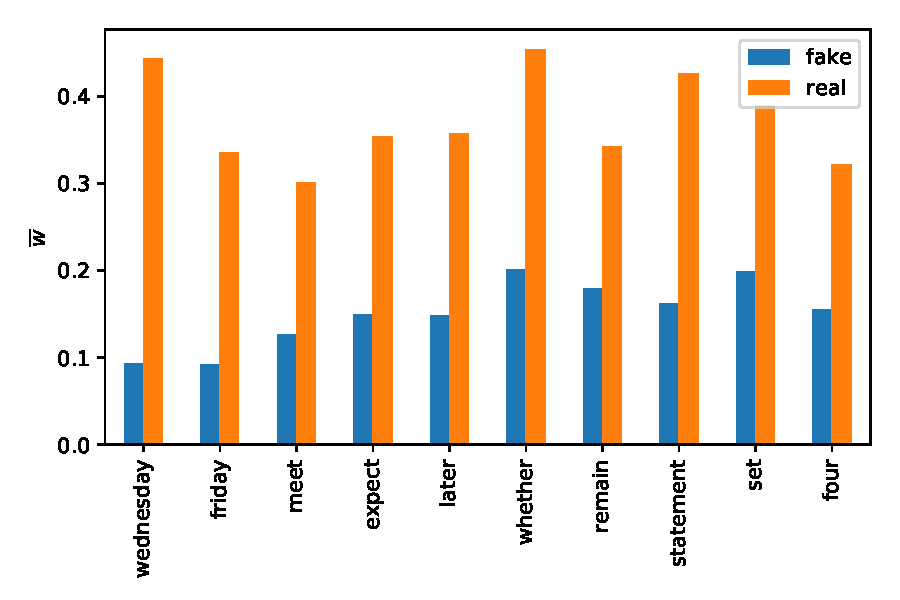
\includegraphics[]{pictures/data_visualisation.pdf}
    \caption{Darstellung der relativen Worthäufigkeit der $10$ Wörter, mit maximaler Differenz der Mittelwerte.
            Eine Unterschied ist klar zu erkennen, wobei ein Teil dadurch erklärt ist, dass die Texte der Real 
            News im Mittel $\approx 1590$ Zeichen länger sind.}
    \label{fig:word_plot}
\end{figure}
Um zu veranschaulichen, ob ein Unterschied der Worthäufigkeiten im Fake- und Real-News Datensatz besteht, werden in \ref{fig:word_plot}
die $10$ Wörter, die am besten zur Trennung geeignet sind, dargestellt. 
Als Kriterium wird 
\begin{equation}
    \frac{(\overline{w_{real}}-\overline{w_{fake}})^2}{s_{real}^2+s_{fake}^2}
\end{equation}
verwendet, welches von der ein dimensionalen linearen Fisher Diskriminanzanalyse inspiriert ist. 
Dabei ist $\overline{w_k}$ das arithmetische Mittel und $s_{k}^{2}=\sum_{i=1}^{N_{k}}\left(w_{k i}-\overline{w}_{k}\right)^{2}$ 
die Summe der quadrierten Abweichungen.
Wörter mit großen Distanzen zwischen den Mittelwerten relativ zu der Streuung können gut zur Trennung genutzt werden.
In \ref{fig:word_plot} ist zu erkennen, dass Real und Fake News durchaus anhand der Worthäufigkeit zu unterscheiden sind. 
Gründe können zum einen Unterschiede in der Ausdrucksweise sein und zum anderen unterschiedliche Themenbereiche. Da die 
Wörter in \ref{fig:word_plot} keine themenspezifischen Worte sind, deutet es daraufhin, dass eher eine unterschiedliche 
Ausdrucksweise ausschlaggeben ist. 
Zum Beispiel scheinen genaue Wochentage in Real News häufiger verwendet zu werden. 
Das kann zum Teil daher bekommen, dass bei Fakten ein genauer Zeitpunkt erwähnt werden kann und bei Falschnachrichten, die 
nur auf eine emotionale Reaktion zielen, ist der genaue Zeitpunkt des Ereignisses nicht existent und auch nicht relevant.
Zu beachten ist, dass Real News im Mittel $\num{1590}$ Zeichen länger sind als Fake News und somit die relative Häufigkeit 
generell bei Real News höher ist als bei Fake News. 
Dies ist jedoch auch ein Attribut was aus dem BoW Modell generiert und genutzt werden kann.
Desweiteren scheinen Stoppwörter, wie "whether", relevant zu sein, weshalb sie mit in die Analyse genommen werden.

Um zu genneralisieren, werden nur die $500$ im Trainingsdatensatz am häufigsten verwendeten Wörter als Attribute 
für die Input-Lage des Deep feedforward Neural Networks verwendet. 
Jedoch wird lieber eine L1-Regularizierung in der ersten hidden Layer verwendet, um ein overfitting zu verhindern, 
anstatt die Anzahl der Wörter zu verringern, da, wie in \ref{fig:word_plot} zusehen, häufig verwendete Wörter nicht 
zwangsweise gut zur Trennung geeignet sein müssen.

Das mit Kears\cite{keras} aufgebaute Netz wird mithilfe der \textsc{hyperas}-Bibliothek\cite{hyperas} optimiert und 
es ergibt sich ein optimaler Classifier, wie er in \ref{fig:NN_structure} dargestellt ist.


\chapter{Ergebnisse}
Loss Epoch (plot)
prob auf training und test (overtraining plot)
Confusion Matrix (plot)
ROC Curve (plot)
Confusion hist (plot) [großer mean sodass von generalisieren gesprochen werden kann]
RF erklären 
ROC Curve vergleich (plot)

\begin{figure}[t!]
    \centering
    \begin{subfigure}[t]{0.49\textwidth}
        \centering
        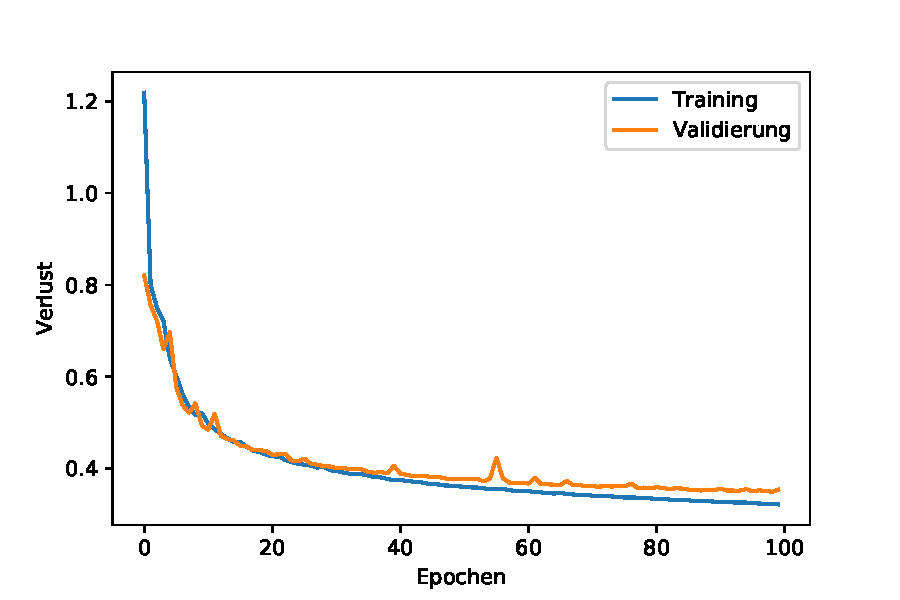
\includegraphics[width=\textwidth]{pictures/history_bow_best.pdf}
        \caption{Abbildung des Trainingsfehler und des Validierungsfehlers im Laufe des Trainings.}
        \label{fig:history}
    \end{subfigure}
    \begin{subfigure}[t]{0.49\textwidth}
        \centering
        \raisebox{1.5cm}[0pt]{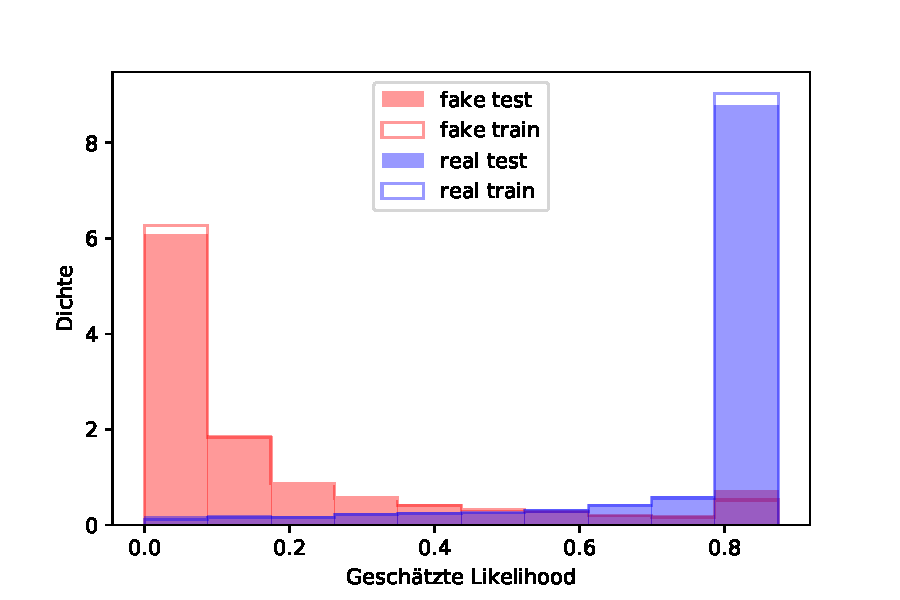
\includegraphics[width=\textwidth]{pictures/prob_bow_best_nn.pdf}}
        \caption{Darstellung der Vorhersage bei Trainings und Testdatensatzes.}
        \label{fig:probs}
    \end{subfigure}
    \caption{Analyse des Modells auf ein mögliches Übertraining, welches }
    \end{figure}

\chapter{Zusammenfassung}
Nur vorhersage für diesen Zeitraum
nur SChreibstil erkennung des BS Filters keine Fake News erkennung 


\chapter{code}
github Link

\appendix
\chapter{Bayesian Optimization}
\chapter{Natural Language Processing}
